\documentclass{article}
\usepackage{eecstex}
\usepackage{physics}
\usepackage{pgfplots}

\renewcommand{\thesubsection}{\thesection.\arabic{subsection}}
\renewcommand{\thesubsubsection}{\thesubsection.\alph{subsubsection}}
\renewcommand{\labelenumi}{\arabic{enumi}.}
\newcommand{\F}{\mathcal{F}}
\newcommand{\sinc}{\operatorname{sinc}}
\newcommand{\rect}{\operatorname{rect}}


\let\Re\relax
\DeclareMathOperator{\Re}{\mathfrak{R}}
\let\Im\relax
\DeclareMathOperator{\Im}{\mathfrak{I}}

\title{EE 120 HW 13}
\author{Bryan Ngo}
\date{2021-04-26}

\begin{document}

\maketitle

\section{Z-Transform Warmup}

By PFD,
\begin{align}
    Z(z) &= \frac{1 - 2z^{-1}}{1 + \frac{5}{2} z^{-1} + z^{-2}} = \frac{1 - 2z^{-1}}{(1 + 2z^{-1}) (1 + \frac{1}{2} z^{-1})} = \frac{A}{1 + \frac{1}{2} z^{-1}} + \frac{B}{1 + 2z^{-1}} \\
    1 - 2z^{-1} &= A (1 + 2z^{-1}) + B \qty(1 + \frac{1}{2} z^{-1}) \\
    z = -2 &\implies B = \frac{8}{3} \\
    z = -\frac{1}{2} &\implies A = -\frac{5}{3} \\
    \implies \frac{1 - 2z^{-1}}{(1 + \frac{1}{2} z^{-1}) (1 + 2z^{-1})} &= -\frac{5}{3} \frac{1}{1 + \frac{1}{2} z^{-1}} + \frac{8}{3} \frac{1}{1 + 2z^{-1}} \\
    \implies z[n] &= -\frac{8}{3} \qty(-\frac{1}{2})^n u[n] + \frac{5}{3} (-2)^n u[n]
\end{align}

\section{Second Order LCCDE}

\begin{equation}
    y[n] - \frac{3}{2} y[n - 1] + \frac{1}{2} y[n - 2] = x[n]
\end{equation}

\subsection{}

\begin{align}
    Y(z) - \frac{3}{2} z^{-1} Y(z) + \frac{1}{2} z^{-2} Y(z) &= X(z) \\
    \implies H(z) &= \frac{1}{2 - 3z^{-1} + z^{-2}}
\end{align}
with ROC \(|z| > 1\).

\subsection{}

We can factor the denominator to be
\begin{equation}
    2 - 3z^{-1} + z^{-2} = 0 \implies z = 1, \frac{1}{2}
\end{equation}
The system is not stable since \(z = 1\) is not inside the unit circle.

\subsection{}

\begin{align}
    X(z) &= \frac{1}{1 - z^{-1}} \\
    Y(z) &= \frac{1}{(2 - z^{-1}) (1 - z^{-1})^2}
\end{align}
Using the fact that
\begin{equation}
    \widetilde{x}[n] = \sum_{k \leqslant n} x[k] \longleftrightarrow \widetilde{x}[n] = \frac{1}{1 - z^{-1}} X(z)
\end{equation}
Then,
\begin{align}
    y[n] = \sum_{\ell \leqslant n} \sum_{k \leqslant \ell} \qty(\frac{1}{2})^k u[k] &= \sum_{\ell \in [0, n]} \sum_{k \in [0, \ell]} \qty(\frac{1}{2})^k u[n] \\
    &= \qty(2 (n + 1) - \sum_{\ell \in [0, n]} \qty(\frac{1}{2})^\ell) u[n] \\
    &= \qty(2 (n + 1) - \qty(2 - \qty(\frac{1}{2})^n)) u[n] = \qty(2n + \qty(\frac{1}{2})^n) u[n]
\end{align}

\section{}

\begin{align}
    Y(z) - \frac{3}{2} (z^{-1} Y(z) + y[-1]) + \frac{1}{2} (z^{-2} Y(z) + z^{-1} y[-1] + y[-2]) &= 0 \\
    (2 - 3z^{-1} + z^{-2}) Y(z) &= \frac{3}{2} y[-1] - \frac{1}{2} z^{-1} y[-1] - \frac{1}{2} y[-2] \\
    Y(z) &= \frac{4 - 3z^{-1}}{2 - 3z^{-1} + z^{-2}} = \frac{1}{1 - \frac{1}{2} z^{-1}} + \frac{1}{1 - z^{-1}} \\
    \implies y[n] = \qty(\qty(\frac{1}{2})^n + 1) u[n]
\end{align}

\section{LTI Transfer Function}

\begin{equation}
    H(z) = \frac{\num{0.05634} (1 + z^{-1}) (1 - \num{1.0166} z^{-1} + z^{-2})}{(1 - \num{0.683} z^{-1}) (1 - \num{1.14461} z^{-1} + \num{0.7957} z^{-2})}
\end{equation}

\subsection{}

\begin{align}
    H(z) &= \frac{\num{0.05634} (1 + z^{-1}) (1 - \num{1.0166} z^{-1} + z^{-2})}{(1 - \num{0.683} z^{-1}) (1 - \num{1.14461} z^{-1} + \num{0.7957} z^{-2})} \\
    &= \frac{\num{0.05634} (z + 1) (1 - \num{1.0166} z + z^2)}{(z - \num{0.683}) (1 - \num{1.14461} z + \num{0.7957} z^2)}
\end{align}
By the quadratic formula, we find that
\begin{align}
    z_1 &= -1 \\
    z_2, z_3 &= \num{0.5083} \pm \num{0.8612j} \\
    p_1 &= 0.683 \\
    p_2, p_3 &= \num{0.7231} \pm \num{0.5224j}
\end{align}

\begin{center}
    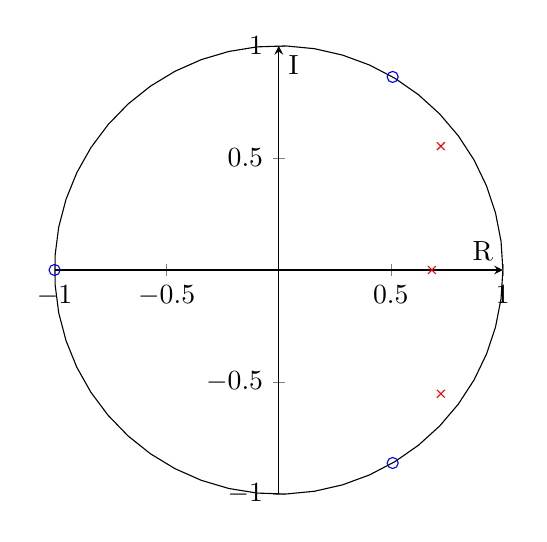
\begin{tikzpicture}
        \begin{axis}[
            xlabel=\(\Re\), ylabel=\(\Im\),
            axis lines=middle,
            axis equal image
        ]
        \addplot[
            only marks,
            color=blue,
            mark=o,
        ]
        coordinates {
            (-1, 0)
            (0.5083, 0.8612)
            (0.5083, -0.8612)
        };
        \addplot[
            only marks,
            color=red,
            mark=x,
        ]
        coordinates {
            (0.683, 0)
            (0.7231, 0.5524)
            (0.7231, -0.5524)
        };
        \addplot [domain=0:2*pi,samples=50]({cos(deg(x))},{sin(deg(x))});
        \end{axis}
    \end{tikzpicture}
\end{center}
The system is stable since all our poles are in the unit disk.

\subsection{}

\begin{center}
    \includegraphics[width=0.8\textwidth]{Screenshot 2021-04-26 at 15-44-44 Files.png}
\end{center}

\section{Band-Pass Filter}

\begin{equation}
    H_{bp}(z) = \frac{1 - \alpha}{2} \frac{1 - z^2}{1 - \beta (1 + \alpha) z^{-1} + \alpha z^{-2}}
\end{equation}

\subsection{}

\begin{align}
    H_{bp}(z) + H_{bs}(z) &= \frac{1 - \alpha}{2} \frac{1 - z^2}{1 - \beta (1 + \alpha) z^{-1} + \alpha z^{-2}} + \frac{1 + \alpha}{2} \frac{1 - 2\beta z^{-1} + z^{-2}}{1 - \beta (1 + \alpha) z^{-1} + \alpha z^{-2}} \\
    &= \frac{(1 - \alpha) - z^2 (1 - \alpha) + (1 + \alpha) - 2\beta z^{-1} (1 - \alpha) + z^{-2} (1 + \alpha)}{2 (1 - \beta (1 + \alpha) z^{-1} + \alpha z^{-2})} \\
    &= \frac{2 - 2 \beta (1 + \alpha) z^{-1} + 2\alpha z^{-2}}{2 (1 - \beta (1 + \alpha) z^{-1} + \alpha z^{-2})} = 1
\end{align}

\subsection{}

\begin{align}
    H_{bp}(e^{j 0}) &= 1 - H_{bs}(e^{j 0}) = 0
    H_{bp}(e^{j \pi}) &= 1 - H_{bs}(e^{j \pi}) = 0
    H_{bp}(e^{j \omega_0}) &= 1 - H_{bs}(e^{j \omega_0}) = 1
\end{align}

\section{System Described by Block Diagram}

\begin{align}
    y[n] &= b_0 x[n] + (b_1 x - a_1 y)[n - 1] + (b_2 x - a_2 y)[n - 2] \\
    &= b_0 x[n] + b_1 x[n - 1] - a_1 y[n - 1] + b_2 x[n - 2] - a_2 y[n - 2] \\
    y[n] + a_1 y[n - 1] + a_2 y[n - 2] &= b_0 x[n] + b_1 x[n - 1] + b_2 x[n - 2] \\
    \implies H(z) &= \frac{b_0 + b_1 z^{-1} b_2 z^{-2}}{1 + a_1 z^{-1} + a_2 z^{-2}}
\end{align}

\end{document}
